% Lebesgue times counting measure on the diagonal: sections of measure 1 one way, 0 the other. Generated by a short script.
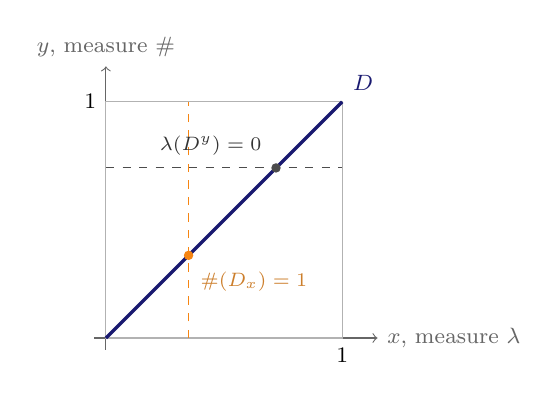
\begin{tikzpicture}[scale=3]
\draw[->,black!60] (-0.05,0) -- (1.15,0) node[right,font=\footnotesize] {$x$, measure $\lambda$};
\draw[->,black!60] (0,-0.05) -- (0,1.15) node[above,font=\footnotesize] {$y$, measure $\#$};
\draw[black!30] (0,0) rectangle (1,1);
\draw[MidnightBlue,very thick] (0,0) -- (1,1) node[above right,font=\footnotesize] {$D$};
\draw[BurntOrange,dashed] (0.35,0) -- (0.35,1);
\fill[BurntOrange] (0.35,0.35) circle (0.02);
\node[font=\scriptsize,BurntOrange!80!black,right] at (0.36,0.24) {$\#(D_x)=1$};
\draw[black!70,dashed] (0,0.72) -- (1,0.72);
\fill[black!70] (0.72,0.72) circle (0.02);
\node[font=\scriptsize,black!80,above left] at (0.7,0.73) {$\lambda(D^y)=0$};
\node[font=\footnotesize,below] at (1,0) {$1$};
\node[font=\footnotesize,left] at (0,1) {$1$};
\end{tikzpicture}
